\documentclass[tikz,border=12pt]{standalone}
\usepackage[T1]{fontenc}
\usepackage{mathpazo}
\usepackage{amsmath,amssymb}
\usetikzlibrary{arrows.meta, positioning, calc, decorations.pathreplacing}

\definecolor{stblue}{HTML}{7B97AD}
\definecolor{rwgold}{HTML}{B8995E}
\definecolor{sage}{HTML}{7A9A7E}
\definecolor{dkbrown}{HTML}{3D3530}
\definecolor{wmgray}{HTML}{7B7067}
\definecolor{cream}{HTML}{F9F6F0}
\definecolor{border}{HTML}{D4C9B8}
\definecolor{terracotta}{HTML}{C47A6A}
\definecolor{lavender}{HTML}{907EA0}

\begin{document}
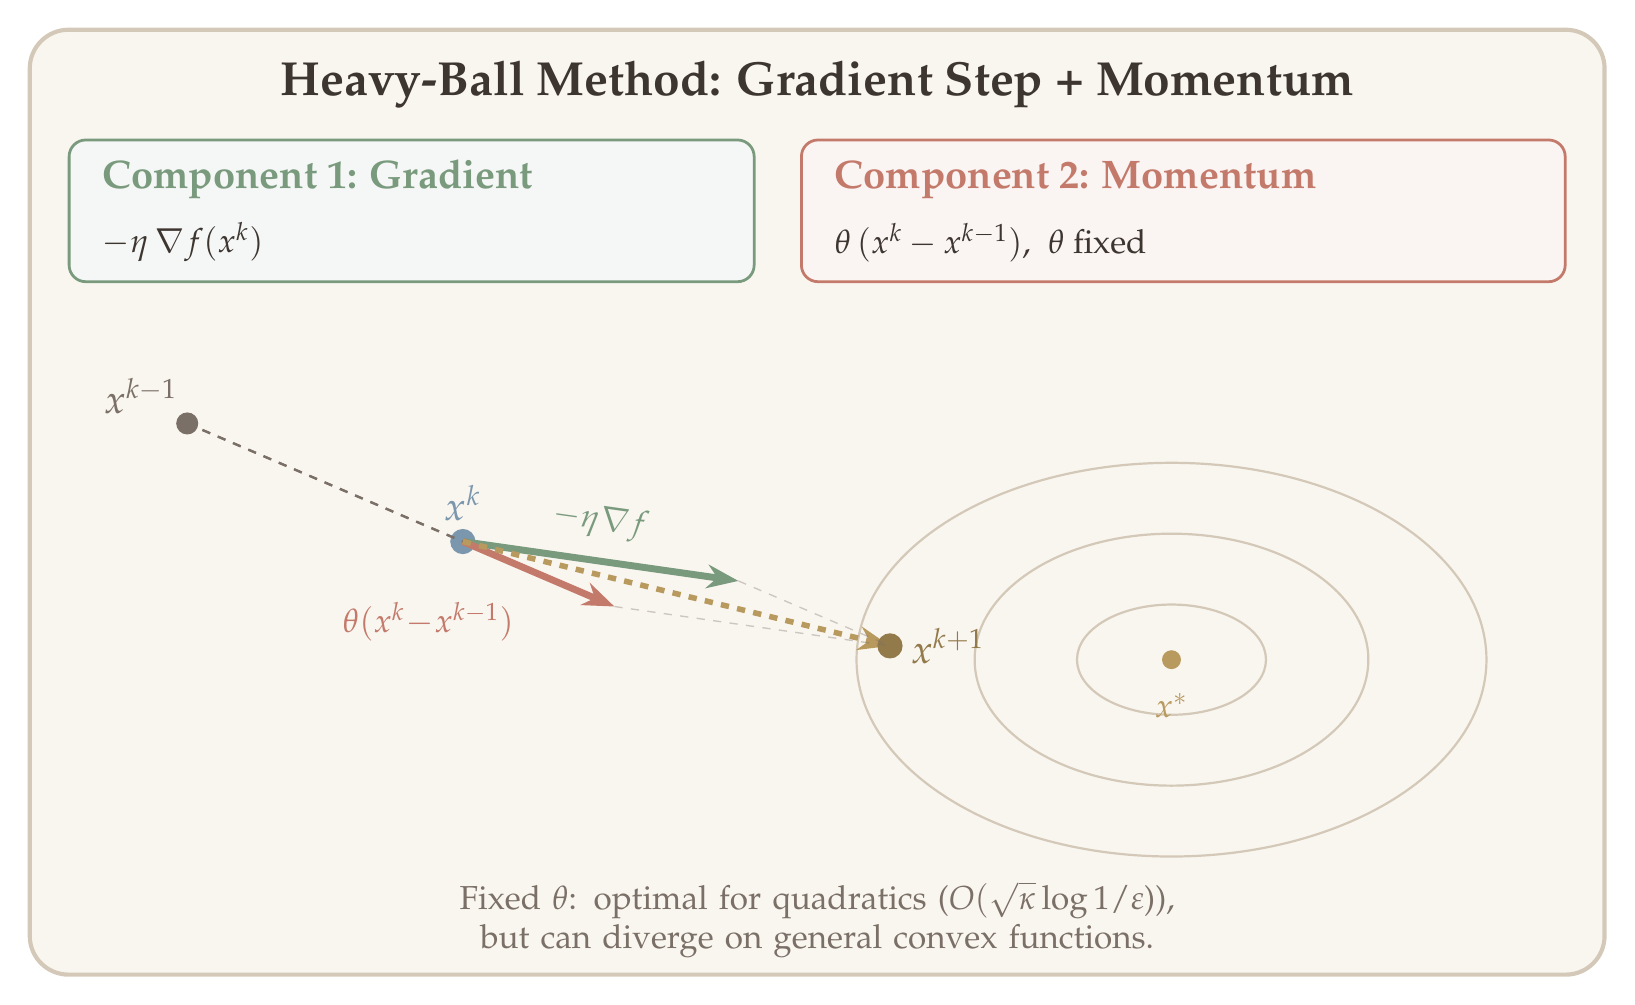
\begin{tikzpicture}[
  >={Stealth[length=4mm, width=3mm]},
  every node/.style={text=dkbrown, font=\large},
]

% Background
\fill[cream, rounded corners=14pt] (0,0) rectangle (20,12);
\draw[border, line width=1.5pt, rounded corners=14pt] (0,0) rectangle (20,12);

% Title
\node[font=\LARGE\bfseries, text=dkbrown] at (10,11.3) {Heavy-Ball Method: Gradient Step + Momentum};

% Legend boxes at top
% Component 1: Gradient
\draw[sage, line width=1pt, rounded corners=6pt, fill=sage!8]
  (0.5,8.8) rectangle (9.2,10.6);
\node[font=\Large\bfseries, text=sage, anchor=west] at (0.8,10.1) {Component 1: Gradient};
\node[font=\large, anchor=west] at (0.8,9.3) {$-\eta\,\nabla f(x^k)$};

% Component 2: Momentum
\draw[terracotta, line width=1pt, rounded corners=6pt, fill=terracotta!8]
  (9.8,8.8) rectangle (19.5,10.6);
\node[font=\Large\bfseries, text=terracotta, anchor=west] at (10.1,10.1) {Component 2: Momentum};
\node[font=\large, anchor=west] at (10.1,9.3) {$\theta\,(x^k - x^{k-1})$, \;$\theta$ fixed};

% Contour ellipses — center-right
\draw[border, line width=0.8pt] (14.5,4.0) ellipse (4.0 and 2.5);
\draw[border, line width=0.8pt] (14.5,4.0) ellipse (2.5 and 1.6);
\draw[border, line width=0.8pt] (14.5,4.0) ellipse (1.2 and 0.7);

% Optimum
\fill[rwgold] (14.5,4.0) circle (0.12);
\node[font=\large, text=rwgold, below] at (14.5,3.7) {$x^*$};

% ======== Key coordinates (all derived consistently) ========
% x^{k-1}
\coordinate (xprev) at (2.0,7.0);
% x^k
\coordinate (xk) at (5.5,5.5);
% Direction: x^k - x^{k-1} = (3.5, -1.5)
%
% Gradient displacement: (3.5, -0.5) — roughly toward optimum
% Momentum displacement: 0.55 * (3.5, -1.5) = (1.925, -0.825)
%
% Gradient endpoint:   xk + (3.5, -0.5)   = (9.0, 5.0)
% Momentum endpoint:   xk + (1.925,-0.825) = (7.425, 4.675)
% Combined x^{k+1}:   xk + (3.5,-0.5) + (1.925,-0.825) = (10.925, 4.175)

\coordinate (grad end) at (9.0, 5.0);
\coordinate (mom end)  at (7.425, 4.675);
\coordinate (xnext)    at (10.925, 4.175);

% --- Previous iterate x^{k-1} ---
\fill[wmgray] (xprev) circle (0.14);
\node[font=\Large, text=wmgray, above left] at (xprev) {$x^{k-1}$};

% --- Current iterate x^k ---
\fill[stblue] (xk) circle (0.16);
\node[font=\Large, text=stblue, above=4pt] at (xk) {$x^k$};

% Dashed line from x^{k-1} through x^k showing previous displacement direction
\draw[wmgray, line width=0.8pt, dashed] (xprev) -- ($(xk)!1.35!($(xk)$)$);
% Actually, extend the line x^{k-1} -> x^k a bit beyond x^k
\draw[wmgray, line width=0.8pt, dashed] (xprev) -- ($(xprev)!1.4!(xk)$);

% --- Gradient step arrow from x^k (sage green) ---
\draw[sage, line width=2.5pt, ->] (xk) -- (grad end);
\node[font=\large\bfseries, text=sage, fill=cream, inner sep=3pt, rotate=-8]
  at ($(xk)!0.5!(grad end) + (0,0.5)$) {$-\eta\nabla f$};

% --- Momentum arrow from x^k (terracotta) — PARALLEL to x^{k-1}->x^k ---
\draw[terracotta, line width=2.5pt, ->] (xk) -- (mom end);
\node[font=\large\bfseries, text=terracotta, fill=cream, inner sep=3pt, anchor=north east]
  at ($(xk)!0.55!(mom end) + (-0.3,-0.2)$) {$\theta(x^k\!-\!x^{k-1})$};

% --- Combined x^{k+1} (gold dashed arrow) ---
\draw[rwgold, line width=2pt, dashed, ->] (xk) -- (xnext);

% x^{k+1} point
\fill[rwgold!80!black] (xnext) circle (0.16);
\node[font=\Large, text=rwgold!80!black, right=4pt] at (xnext) {$x^{k+1}$};

% Parallelogram completion: faint dashed lines
\draw[wmgray, line width=0.5pt, dashed, opacity=0.35] (grad end) -- (xnext);
\draw[wmgray, line width=0.5pt, dashed, opacity=0.35] (mom end) -- (xnext);

% Bottom annotation
\node[font=\large, text=wmgray, text width=17cm, align=center] at (10,0.7)
  {Fixed $\theta$: optimal for quadratics ($O(\sqrt{\kappa}\log 1/\varepsilon$)), but can diverge on general convex functions.};

\end{tikzpicture}
\end{document}
